\documentclass{article}
\usepackage{graphicx} % Required for inserting images
\usepackage[utf8]{inputenc}
\usepackage{polski}
\usepackage[dvipsnames]{xcolor}
\usepackage{indentfirst}
\usepackage{multicol}
\usepackage{geometry}
\usepackage{titlesec}
\usepackage[colorlinks=true, linkcolor=gray, urlcolor=blue, citecolor=green]{hyperref}
\usepackage{makecell}
\usepackage{float}
\usepackage[polish]{babel}
\usepackage[T1]{fontenc}
\usepackage[justification=centering]{caption}
\usepackage[utf8]{inputenc} 
\usepackage{subfig}


\usepackage{mwe} % for 'example-image'
\usepackage{newfloat}
\DeclareFloatingEnvironment{graph}
\addto\captionspolish{%
  \renewcommand{\graphname}{Wykres}%
  \renewcommand{\figurename}{Rysunek}%
  \renewcommand{\tablename}{Tabela}%
}


\begin{document}

\begin{titlepage}
    \begin{center}
        \vspace*{1cm}
            
        \Huge
        \textbf{Sprawozdanie z laboratorium 5}
            
        \vspace{0.5cm}
        \LARGE
        IO-LINK (S7-1200) 
            
        \vspace{1.5cm}
            
        \textbf{Łukasz Janusz\\Marek Generowicz}

        \normalsize      
        \textcolor{gray}{13.03.2025}
        \vfill
        \begin{figure}[hb]
            \centering
            
\includegraphics[width=0.5\textwidth]{media/Logo_AGH.jpg}
        \end{figure}   
    \end{center}
\end{titlepage}

\section{Wstęp}
Na laboratoriach należało zapoznać się z cyfrowym, szeregowym protokołem komunikacyjnym IO-Link oraz jego konfiguracją w sterowniku S7-1200. Protokół ten jest szeroko używany w przemyśle do komunikacji sterowników z urządzeniami peryferyjnymi. IO-Link jest systemem typu point-to-point, co oznacza że każde urządzenie jest połączone bezpośrednio z masterem. IO-Link pozwala na łączenie się z urządzeniami analogowymi i cyfrowymi, a także może zostać użyty jako zasilanie. Ze względu na swoją specyfikę, stosowany jest głównie w warunkach lokalnych. 

\section{Opis Stanowiska}
Na stanowisku laboratoryjnym (Zdjęcie \ref{fig:stanowisko}) znajdował się sterownik S7-1200 marki Siemens wyposażony w czterokanałowy moduł IO-Link. Do sterownika podłączono ultradźwiękowy czujnik odległości UGT205. Zestaw uzupełniały kontrolki LED w kolorze niebieskim i białym. 

\begin{figure}[H]
    \centering
    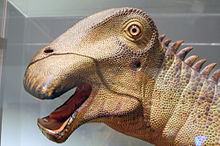
\includegraphics[width=1\textwidth]{media/Brak_zdjecia.png}
    \caption{Stanowisko laboratoryjne (zdjęcie z instrukcji)}
    \label{fig:stanowisko}
\end{figure}

\newpage
\section{Przebieg ćwiczenia}
Aby wykonać ćwiczenie należało wykonać następujące kroki:
\begin{itemize}
    \item konfiguracją sterownika
    \item programowanie S7-PCT (Port Configuration Tool)
    \item odczyt danych z PLC
\end{itemize}

\subsection{Konfiguracja sterownika}
Po poprawnym skonfigurowaniu CPU oraz M 1278 4xIO-Link master z programem TIA Portal V19, otrzymywało się wirtualny odpowiednik stanowiska laboratoryjnego. Wygląd w programie TIA Portal przedstawiono na zdjęciu \ref{fig:konfiguracja}.

\begin{figure}[H]
    \centering
    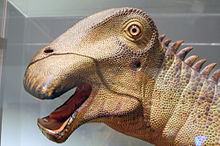
\includegraphics[width=0.8\textwidth]{media/Brak_zdjecia.png}
    \caption{Schemat stanowiska w programie TIA Portal}
    \label{fig:konfiguracja}
\end{figure}

Aby dokończyć konfiguracje należało przeprowadzić identyfikacje sprzętową modułu dla portu pierwszego oraz przesłać konfiguracje do sterownika. Po zakończeniu konfiguracji należało przejść do programowania S7-PCT.

\newpage
\subsection{Programowanie S7-PCT}
Aby rozpocząć należało kliknąć moduł IO-LINK prawym przyciskiem myszy a następnie wybrać \textit{Start Device Tool}. Otwarło się wtedy okno przedstawione na zdjęciu \ref{fig:Dev_tool}

\begin{figure}[H]
    \centering
    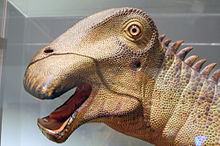
\includegraphics[width=0.8\textwidth]{media/Brak_zdjecia.png}
    \caption{Okno Device Tool}
    \label{fig:Dev_tool}
\end{figure}

Następnie należało przejść do zakładki status i połączyć się z urządzeniem wynikiem czego powinno wyświetlić się kno jak na zdjęciu \ref{fig:status}.

\begin{figure}[H]
    \centering
    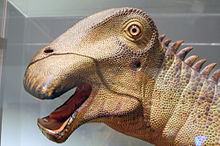
\includegraphics[width=0.8\textwidth]{media/Brak_zdjecia.png}
    \caption{Okno statusu po pomyślnym nawiązaniu połączenia.}
    \label{fig:status}
\end{figure}

\newpage

W następnej kolejności należało przejść do zakładki \textit{Adresses}, a w nim zaznaczyć \textit{Show PLC addresses} oraz \textit{All ports}.
Umożliwia to odczyt adresów zmiennych procesowych urządzenia w PLC. Na rysunku \ref{fig:adresy}.

W programie dostajemy cztery outputy, które oznaczają odpowiednio: 
\begin{itemize}
    \item \textbf{PDV 1}(int) - odległość od czujnika w milimetrach
    \item \textbf{OUT 1}(bool) - status \textit{Swiching Signal Channel 1}
    \item \textbf{OUT 2}(bool) - status \textit{Output Configuration 2}
    \item \textbf{Device Status}(byte) - bajt statusowy
\end{itemize}


\begin{figure}[H]
    \centering
    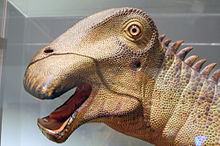
\includegraphics[width=0.8\textwidth]{media/Brak_zdjecia.png}
    \caption{Okno adresów}
    \label{fig:adresy}
\end{figure}
\newpage

\subsection{Odczyt danych z PLC}
nic

\end{document}
